\documentclass[conference]{IEEEtran}
\IEEEoverridecommandlockouts

\usepackage[utf8]{inputenc}

\usepackage{cite}
\usepackage{amsmath,amssymb,amsfonts}
\usepackage{algorithmic}
\usepackage{graphicx}
\usepackage{textcomp}
\usepackage{xcolor}
\usepackage{siunitx}
\usepackage{hyperref}
\usepackage[noabbrev, capitalize]{cleveref}
\usepackage{bm}
\usepackage{todonotes}
\usepackage{tabu}
\usepackage{booktabs}
\usepackage{subfig}

\begin{document}

\title{Lidar to end-effector calibration approach\\ using planar based features}

\author{\IEEEauthorblockN{Bernardo Lourenço}
\IEEEauthorblockA{\textit{Departamento de Engenharia Mecânica} \\
\textit{Universidade de Aveiro}\\
Aveiro, Portugal \\
bernardo.lourenco@ua.pt}
\and
\IEEEauthorblockN{Miguel Riem Oliveira}
\IEEEauthorblockA{\textit{Departamento de Engenharia Mecânica} \\
\textit{Universidade de Aveiro}\\
Aveiro, Portugal \\
mriem@ua.pt}
\and
\IEEEauthorblockN{Paulo de Jesus Dias}
\IEEEauthorblockA{\textit{IEETA} \\
\textit{Universidade de Aveiro}\\
Aveiro, Portugal \\
paulo.dias@ua.pt}
}

\maketitle

\begin{abstract}
The LRF is an essential sensor in the field of robotics, providing accurate range measurements with high angular resolution. This sensors are also popular in 3D reconstruction systems, mounted in kinematic chains, such as PTUs. However, the extrinsic transformation of the LRF has to be determined with high accuracy, otherwise the 3D reconstructions will be unusable for any subsequent procedure. In this work, a calibration procedure which determines this transformation is described which promises high accuracy and requires no external markers. This method was evaluated using real 3D reconstruction data, and proved to be successful in finding the correct transformation. 
\end{abstract}

\begin{IEEEkeywords}
LRF, calibration, reconstruction, point cloud, optimization
\end{IEEEkeywords}

\section{Introduction}\label{section:introduction}

The Laser Range Finder, or LRF, is one of the most important sensors in the field of robotics, employed in applications such as SLAM~\cite{wang14,eyice18} and 3D reconstruction~\cite{klimentjew10,saito10}. Its use is increasing due to their continuously decrease in price, new research and development and its fundamental role in emerging technologies such as autonomous driving.

In this paper, a 2D LRF is used in a 3D reconstruction system, to produce high-detail and accurate models of real scenes. The common solution involves the integration of the LRF on a robotic arm, such as a PTU, to enable a full 3D reconstruction. However, one of the challenges of this approach is the calibration of the position of the LRF, relative to the coordinate frame of the robotic arm. This process is known as the LRF extrinsic calibration.

This calibration is utterly necessary because any error on it introduces a shift on the position of each point, which in turn can be seen as deformations on the point cloud resulting from the reconstruction, as can be seen in \cref{fig:deformed-pointcloud}. This deformations have a significant impact on subsequent point cloud processing methods, that rely on the accurate representation of the 3D environments, i.e. registration (for example, ICP), segmentation and feature extraction algorithms. 

\begin{figure}[h]
    \centering
    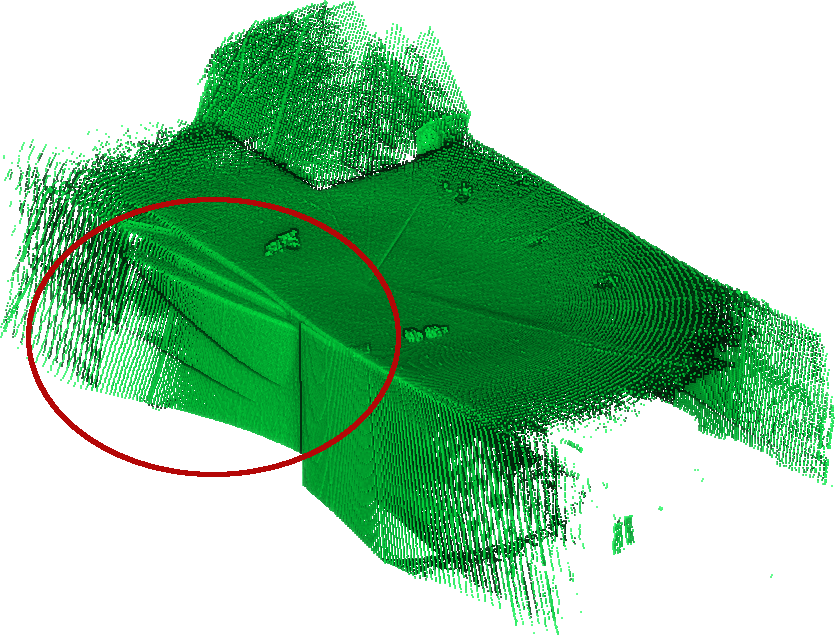
\includegraphics[width=8cm]{images/bad-pointcloud.png}
    \caption{Example of deformed point cloud, product of an inaccurate calibration of the LRF. The points where this deformation is most visible is marked in red.}
    \label{fig:deformed-pointcloud}
\end{figure}

Typically, the standard procedure to do this calibration relies on a study of the geometry of such a system, using a measuring instrument, for example, a tactile Coordinate Measuring Machine. However, this approach has several disadvantages: it is time-consuming, the instruments required are expensive and generally not easily available. Therefore, this solution is often not feasible for research work and prototype development.

Therefore, reliable and automatic methods for the LRF extrinsic calibration are required. In this field, there are two big approaches, depending on the sensor which the LRF is calibrated relative to. The first method, and the most studied, is the calibration of the LRF relative to a camera~\cite{chen16,kassir10,zhang04}, or cameras~\cite{haeselich12}. In this method, the static transformation between these two sensors is determined, and relies on a correspondence between visual features captured by the camera and geometric features captured by the LRF. This features are usualy captured from markers placed on the field of view of both sensor, such as a chessboard, in the case of \cite{kassir10}. However, this methods have some disadvantages in the case of LRF mounted on robotic arms: first, they require the inclusion of a camera in the system; secondly, the calibration of the camera has to be performed; and lastly, the error of both calibrations is combined during the reconstruction, which increases the inaccuracies of the final reconstruction. 

Another approach is the calibration without the use of a camera, but instead the calibration is done against the robotic arm~\cite{zeng18}. Most of these methods rely on the comparison between the structure of the reconstructed points with known geometry, e.g. a marker. In~\cite{kim13}, a marker formed by two perpendicular planes is used, and their points are segmented from the reconstructed point cloud. Then, the relation between the normals of these planes is used as the objective function for the calibration. However, this method presents some limitations: first, ensuring that two planes are perpendicular with a small error can be very hard (cardboard ); second, it is not straight-forward how to increase the number of planes; finally, by using a small marker, only a small portion of the space is occupied, which means that only a portion of the sensors' full field of view is used, which may lead to a sub-optimal result.

In this paper, a new method for the extrinsic calibration of an LRF w.r.t. a robotic arm is presented, which makes use of the reconstructed scene geometry, more specifically, its planar regions. Then, the evaluation of this regions serves as the objective function for an optimization procedure, which searches the position of the LRF which minimizes the deformations of the reconstructed geometry. Results will show that the proposed approach is capable of generating accurately reconstructed scenes.

% TODO:
The remainder of this paper will be structured as follows...

\section{Problem Formulation}\label{section:problem-formulation}

The LRF is a sensor that outputs several laser scans. Each laser scan is a set of range measurements taken along several directions but at the same time, all coincident with a plane, the scan plane. That is in fact why these equipment have a 2D nature. Thus, for each scan, a 2D slice of the scene is measured. Since the LRF is mounted on top of an actuated kinematic chain (e.g. a PTU or robotic manipulator), the movement of this chain positions the LRF in different poses in the 3D space. Through the accumulation of the several laser scans, a dense point cloud of the scene is produced. 

The process of accumulation is, in essence, based on the concatenation of 3D points from multiple scans. However, the grouping of these points requires that the points of each laser scan are transformed to a common, static, reference frame, the map frame. In order to achieve this, one must apply a geometric transformation to each 3D point $\mathbf{q}^{(i)}$ measured in scan $i$, represented in the LRF's local coordinate system $l$. The transformed point $\mathbf{p}^{(i)}$, defined in the map reference frame, is determined by:
%
\begin{equation}\label{equation:point-reconstruction}
    \mathbf{q}^{(i)} = \, ^{m}\mathbf{T}_{e}^{(i)} \cdot ^{e}\mathbf{T}_{l} \cdot \mathbf{p}^{(i)},
\end{equation}
%
\noindent where ${^{m}\mathbf{T}_{e}}^{(i)}$ is the transformation between the map and the end effector coordinate frames, which is dynamic and given by the process that receives a description of the kinematic chain, the joint values at the scan $i$, and computes the direct kinematics. In turn, $^{e}\mathbf{T}_{l}$ denotes the position of the LRF w.r.t the end effector. In the end, the set of all the points $\mathbf{p}$ is denoted as the reconstructed point cloud $\mathcal{P}$.

Note that, although this transformation is static, it influences the coordinates of the points $\mathbf{p}^{(i)}$, and therefore is crucial to the accuracy with which three-dimensional objects are represented in the accumulated point cloud $\mathcal{P}$.
Thus, an accurate estimation of transformation $^{e}\mathbf{T}_{l}$ is paramount to the process of 3D reconstruction. We refer to this procedure of estimation the LRF to end effector transformation, as the Lidar to end-effector extrinsic calibration.

In this work, we propose a novel approach to perform Lidar to end-effector extrinsic calibration. The approach is based on an optimization procedure which computes the transformation that generates planar point cloud sections in areas which are marked as planes. To this end, several existing scene structures may be used, such as walls, ceilings or pavements. This is an additional advantage of our proposed method: it does not require dedicated calibration targets.

%%%%%%%%%%%%%%%%%%%%%%%%%%%%%%%%%%%%%%%%%%%%%%%%%%
\section{Proposed Approach}
\label{section:proposed_approach}
%%%%%%%%%%%%%%%%%%%%%%%%%%%%%%%%%%%%%%%%%%%%%%%%%%

The working principle of this method relies on the following assumption: in a good calibration, the deviation of a measured point set w.r.t. to the real scene geometry should be minimal. This paper focuses on planar geometries because of two reasons:  they are easily segmented from the full point cloud, and it is straightforward to compute a similarity metric between the point cloud and the expected planar geometry. In other words, in a point set representing a planar surface, the deviation from the points to the planar surface should be the lowest, if the calibration is correct.

This method can then be formulated as an optimization problem: for each extrinsic calibration transformation $\mathbf{T}$, corresponds a point cloud $\mathcal{P}$. This point cloud is evaluated by a cost function, which determines quantitatively how good each generated point cloud is. Finally, an optimizer will find the transformation $T$ that minimizes the loss function. Therefore, this method can be defined as:
%
\begin{equation}
    \mathbf{\mathbf{x}} = \underset{\mathbf{x}}{\mathrm{argmin}} \left\{ \mathrm{f}(\mathcal{P}) \right\},
\end{equation}
%
\noindent where $\mathrm{f}$ is the cost function, $\mathcal{P}$ is the resulting point cloud and $x$ are the parameters that define $\mathbf{T}$.

To further explain this method, an explanation of it in each of its components will be done: the parametrization, the cost function and the optimizer. Each of this components are orthogonal to the others so they can be understood independently.

The optimization algorithm chosen was the Powell's method, described in \cite{powell64}. This method finds a local minimum of a multi-dimensional unconstrained function, and does not require the gradient of this function (is unknown in this problem), which fits this particular optimization. This method is implemented in the python scientific library SciPy. However, this method requires multiple evaluations of the objective function at each iteration, in order to calculate a approximate Jacobian matrix in the neighborhood of each point. This usually reflect on slow optimizations, compared to other methods, such as the Gradient Descent.

\subsection{Parametrization}

The parameters in this calibration are six values that define a geometric transformation in space, which is, in the end, cast back to the transformation matrix $\bm{T}$. This transformation is decomposed into two components, a translation, and a rotation. The translation can be represented as the translation vector $\mathbf{t} = \left[t_x, t_y, t_z\right]$, and the rotation is be represented as a $3 \times 3$ rotation matrix $\bm{R}$. Since a rotation matrix has only $3 \times 3 = 9$ elements but only 3 degrees of freedom, another parameterization has to be used to represent a rotation. Popular parameterizations for rotations are Euler angles, quaternions e and axis/angle. However, not all representations are suitable for the optimization procedure. In fact, in~\cite{hornegger99} the term fair parameterization was introduced: a parameterization is called fair if it does not introduce more numerical sensitivity than the one inherent to the problem itself. Therefore, fair parameterizations are required for optimizations, as they increase the chances for convergence. For example, Euler angles, which are probably the most used angle parameterizations, are not suitable~\cite{schmidt01}, because they do not yield smooth movements. Each rotation is non-unique and, most notably, there are singularities, so-called \textit{gimbal-lock} singularities, where one degree of freedom is lost~\cite{schmidt01}. Also, quaternions are not suitable for optimizations, because quaternions have $4$ components which are constrained to a unitary length. Despite being a fair parameterization, quaternions introduce some complexity in the algorithm to handle this constraint, so they are not usually used for optimizations~\cite{schmidt01}.

The axis/angle parameterization is the most widely used to represent a rotation in optimization procedures, as it is a fair parameterization and has only three components. Any rotation can be represented as a rotation around an axis $a$, by an angle $\theta$. Since $\bm{a}$ only represents the direction of the rotation (hence only has 2 degrees of freedom), it can be combined with the angle $\theta$ into a single rotation vector $\bm{\omega} = \left[\omega_1, \omega_2, \omega_3\right]$, as follows:

\begin{equation}
    \label{eqn:axis-angle}
    \begin{aligned}
        \theta & = |\bm{\omega}| \\
        \bm{a} & = \frac{\bm{\omega}}{|\bm{\omega}|}
    \end{aligned}
\end{equation}

Computing the rotation matrix from $\omega$ is done using the Rodrigues' formula~\cite{schmidt01}:
%
\begin{equation}
    \textbf{R} = \bm{I} + \frac{\sin \theta}{\theta} \bm{\Omega} + \frac{1 - \cos \theta}{\theta^2} \bm{\Omega},
\end{equation}
%
\noindent
where I is the $3\times3$ identity matrix, and $\bm{\Omega}$ is given by:
%
\begin{equation}
    \bm{\Omega} = \left[
        \begin{array}{ccc}
            0  & -\omega_3 & \omega_2 \\
            \omega_3 & 0   & -\omega_1 \\
            -\omega_2 & \omega_1 & 0 \\
        \end{array}
    \right].
\end{equation}


In conclusion, the parameter vector to be optimized will have six values: three representing the translation $\bm{t}$ and the rotation vector $\bm{\omega}$ represented in the axis/angle representation. So, the parameter vector $\bm{x}$ is defined as:

\begin{equation}
    \bm{x} = \left[t_1, t_2, t_3, \omega_1, \omega_2, \omega_3\right].
\end{equation}

This optimization was quite robust to the initial parameters, so the first guess was always a null translation and the rotation was done doing a visual inspection of the laser scanner, using angles multiples of \SI{90}{\degree}.

\subsection{Cost Function}

The cost function is a function used in optimization procedures that measures the difference of the result of a model and its expected result. It then yield a value that quantitatively describes the dissimilarity between the two. In this case, the cost function evaluates the distance of each point $\mathbf{p}$ in the point cloud $\mathcal{P}$ to their respective plane. The greater this value, the greater the deformation of the point cloud, and thus the worst the calibration is. This objective is, then, to find the set of parameters that minimize the cost function.

As an initial step, the segmentation of the point cloud is performed. The segmentation is a procedure that divides the point cloud $\mathcal{P}$ into multiple clusters $\mathcal{C}_i$, each one correspondent to different planes on the scene. This segmentation is done prior to the calibration procedure, using the point cloud reconstructed using an initial estimate. Also, this segmentation was done manually because most segmentation algorithms, for example the RANSAC algorithm, were not capable of achieving a reliable segmentation, because the point cloud had significant deformation. In addition, manual segmentation is easy to do and accurate, considering that it is a one-time process. 

During the optimization, this segmentation serves as a blueprint for all segmentations. Each point cloud is generated in the same way, so the sequence of points is always the same. Therefore, it is always possible to match any point on the generated point cloud to the point in the segmented point cloud, and get the corresponding cluster index for all the points. 

\begin{figure}[h]
    \centering
    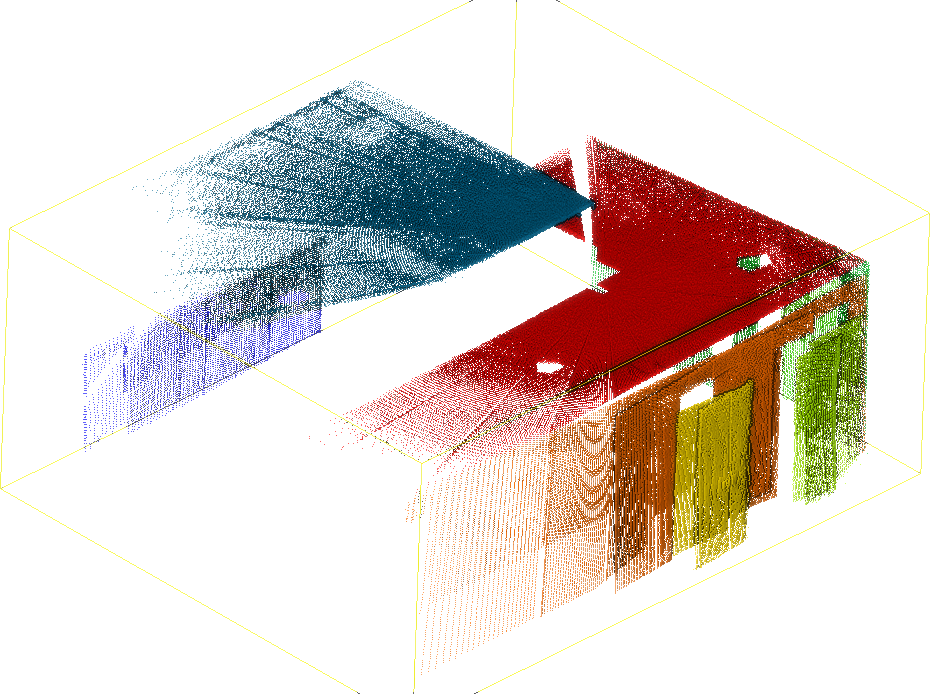
\includegraphics[width=8cm]{images/segmented-pointcloud}
    \caption{Example of a plane segmentation, where each color represents a cluster.}
    \label{figure:cluster-segmentation-1}
\end{figure}

After the segmentation, the calibration procedure can be performed. In an initial step, the plane equation for each point cluster is computed, using the Principal Component Analysis method, or PCA. First the centroid $\bar{p}$ of each plane is found, which is the same as the mean value of all the points $p: (x, y, z) \in \textbf{R}^3$:

\begin{equation}
    \bar{p} = \sum_{i}{p_i}.
        \label{eqn:centroid-plane}
\end{equation}

Then, the covariance matrix $\mathcal{C}$ is calculated:

\begin{equation}
    \mathcal{C} = \sum_{i}{(p_i - \bar{p}) \otimes (p_i - \bar{p})} \footnote{$\otimes$ is the outer tensor product.}.
        \label{eqn:covariance-matrix}
\end{equation}

Then, the principal axes of the plane is find by an eigen-decomposition of the covariance matrix. The smallest eigenvalue $\lambda_3$ will be the variance $\sigma^2$ of the cluster. In other words, $\sigma^2$ is the mean square of the orthogonal distance of all points in the cluster to the plane. So, $\sigma^2$ can be a quantitative factor to measure the cost or each cluster. Formally, let us admit that the $\sigma^2$ has two components: the statistical error of the laser sensor $\sigma^2_{sensor}$, which is not affected by the calibration and a second component $\sigma^2_{calib}$, which depends of the calibration error. Thus, the idea is that, by minimizing $\sigma^2$, a exact calibration can be obtained. For this calibration, however, the value $\sigma$ was used instead of $\sigma^2$, which is known as the Root Mean Square Deviation, or RMS. Therefore, the loss of each cluster will be the $\sigma$ value.

Finally, the scores of the clusters are combined into a scalar value, which is the error of the point cloud. The method found was to, again, calculate the RMS of the values of the partial losses of each cluster $\sigma_i$, according to:
%
\begin{equation}
    \textrm{f} = \sqrt{\sum_{i}^{N}{\sigma_i^2}}.
\end{equation}
%
\noindent This value is expected to be minimal when all the partial losses are minimal which, according to this hypothesis, corresponds to a correct calibration.

%%%%%%%%%%%%%%%%%%%%%%%%%%%%%%%%%%%%%%%%%%%%%%%%%%
\section{Results}
\label{section:results}
%%%%%%%%%%%%%%%%%%%%%%%%%%%%%%%%%%%%%%%%%%%%%%%%%%

In this section, the proposed method for the calibration will be evaluated using acquired data from a real scene. The infraestructure used to acquire the data, as well as a description of the data will be done. Afterward, both a qualitative and quantitative analisys of the results will be performed, to determine how much the geometry of the calibrated point cloud improved, compared to the uncalibrated point cloud. 

The hardware infrastructure used in this work to acquire the data was the 3D scanner \textit{lemonbot}, show in \cref{figure:lemonbot}. The principal components of this 3D scanner are the PTU \textit{FLIR PTU-D46} and the LRF \textit{Hokuyo UTM30LX}. The LRF was mounted on the PTU, to have the scan plane in the vertical direction. The LRF can cover \SI{270}{\degree} with an angular resolution of \SI{0.25}{\degree}. The PTU has an angular resolution of \SI{0.0032}{\degree}, so the error in the transformation $^{m}\mathbf{T}_{e}$ (see \cref{equation:point-reconstruction}) is negligeble. This 3D scanner was programmed using the \textit{ROS} framework, which is handles the hardware drivers, the transformation graph and the recording of the scanning data.

\begin{figure}[h]
    \centering
    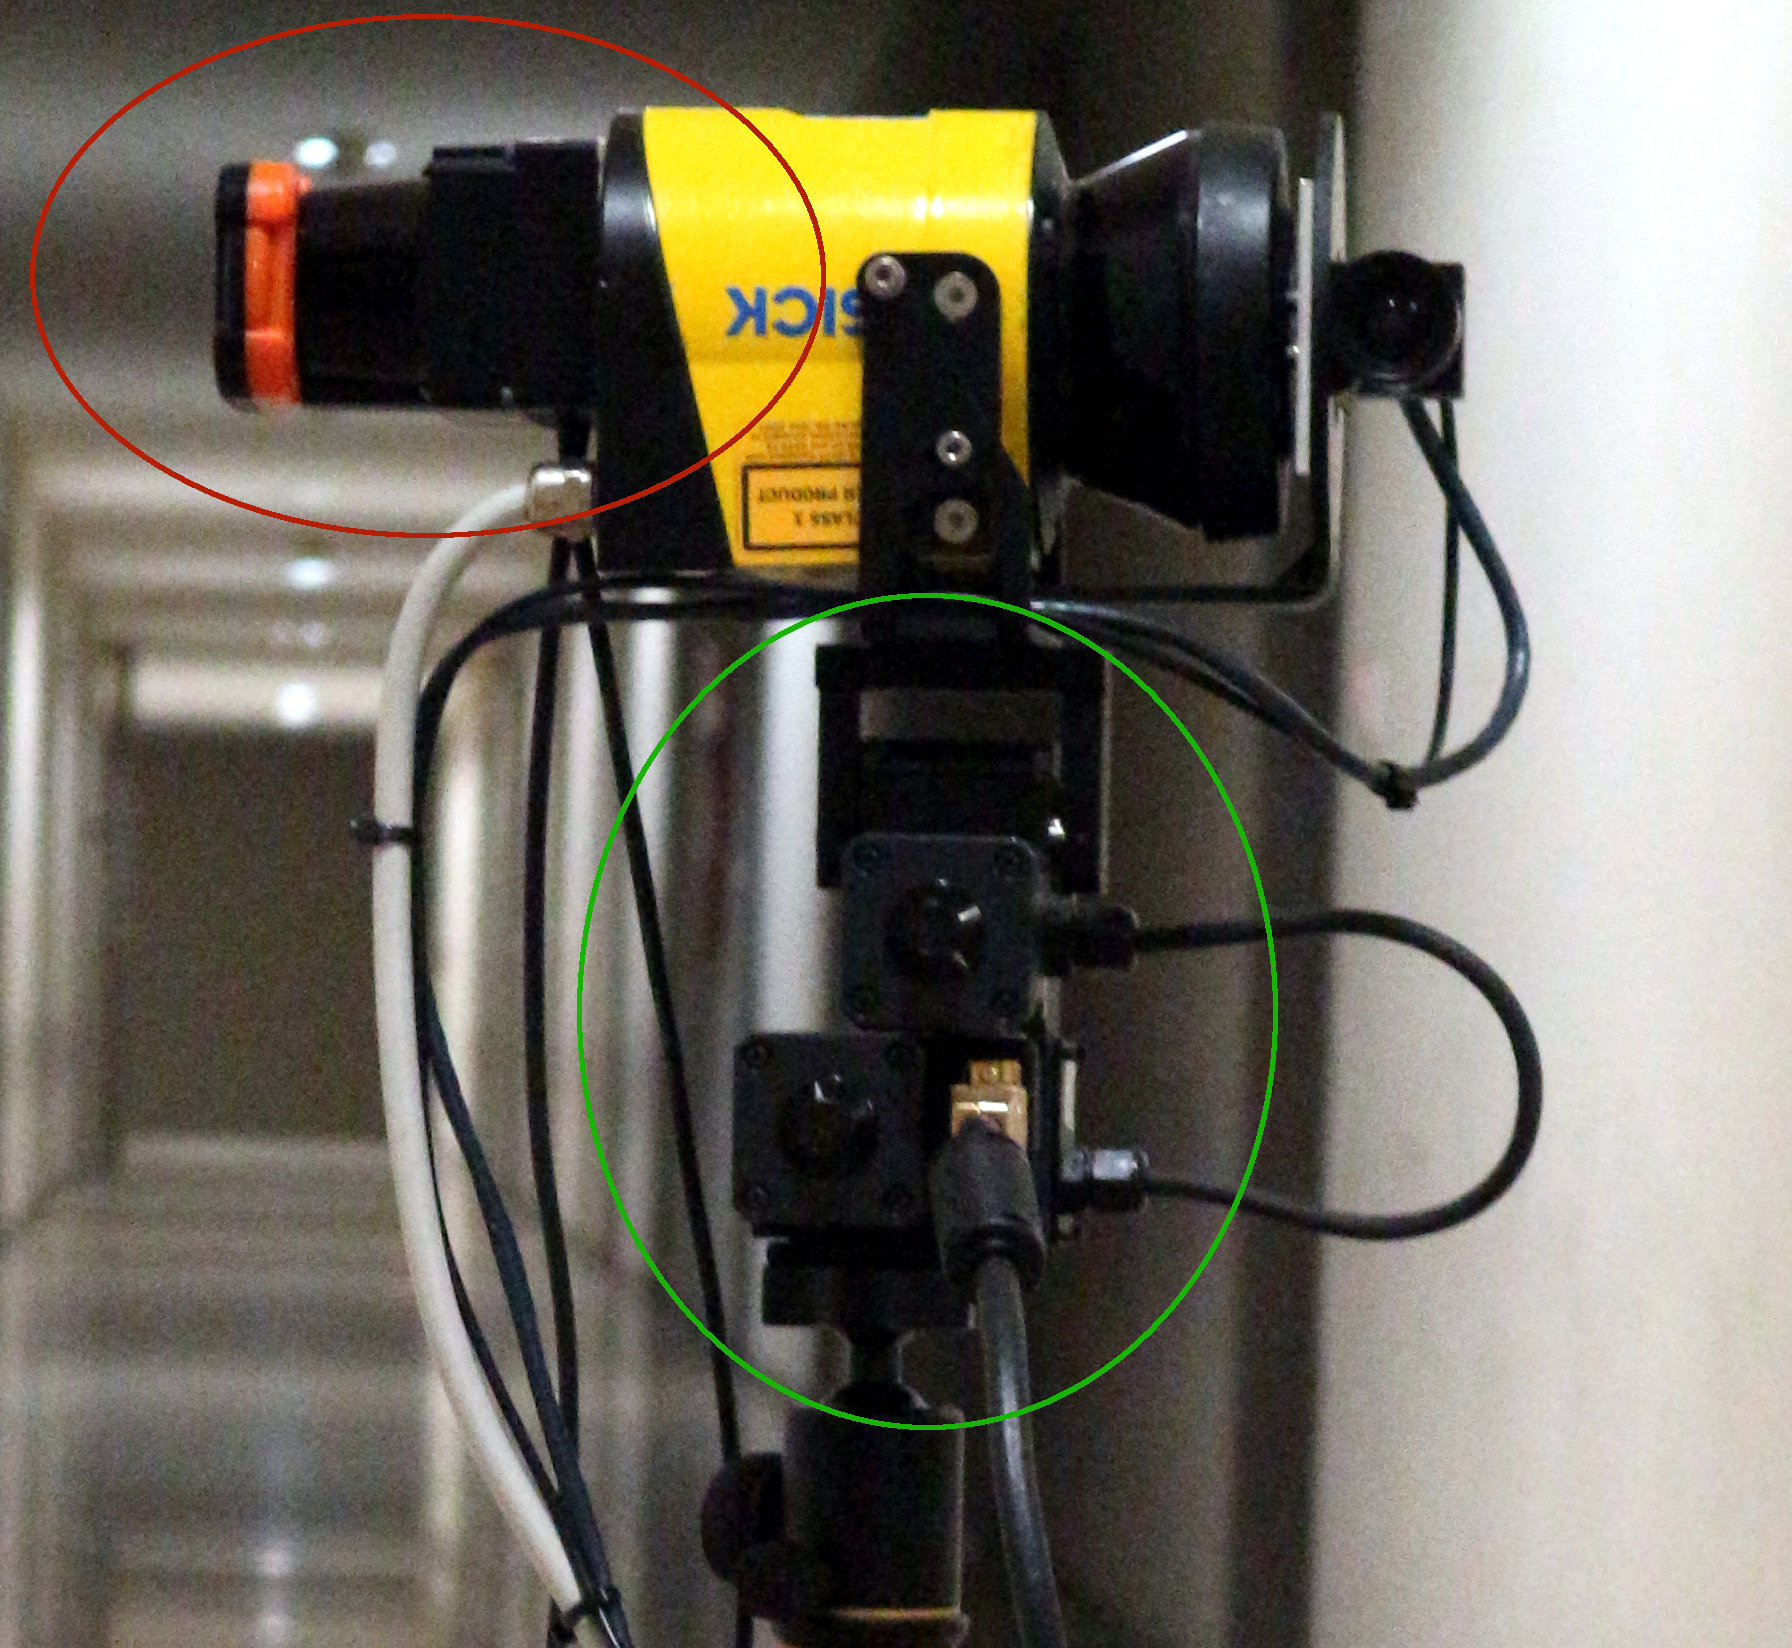
\includegraphics[width=8cm]{images/lemonbot-head}
    \caption{The \textit{lemonbot} 3D scanner, used in this work. The LRF \textit{Hokuyo UTM30} is marked in red and the \textit{FLIR PTU-D46} is marked in green.}
    \label{figure:lemonbot}
\end{figure}

For the verification, a set of 3 datasets was acquired from a single room, which corresponds to 3 point clouds. The acquisitions were performed in different positions in the room. The room was not cluttered and the ceiling, walls and floor are all perpendicular and known to be planar surfaces. This was ensured in order to minimize the segmentation and calibration errors.

The optimization procedure was successful in minimizing the objective function in every dataset, as seen in \cref{table:iteration-results}. The final results a qualitative improvement in comparison to the uncalibrated point cloud, as show in \cref{figure:visual-comparison}. The deformation found in the uncalibrated point cloud are almost imperceptible in the calibrated point cloud.

\begin{figure}
    \centering
    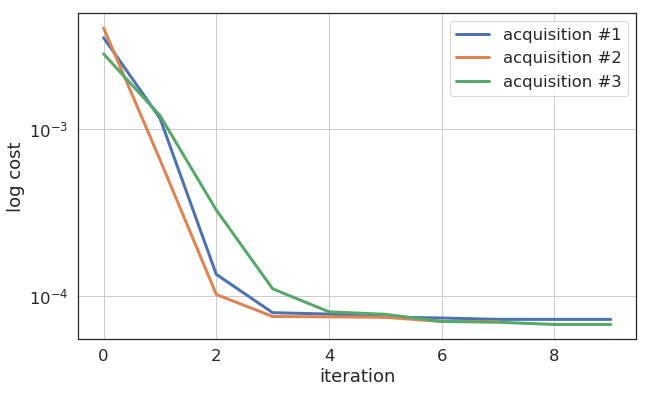
\includegraphics[width=8cm]{images/calibration-evolution.png}
    \caption{Graph of the evolution of the cost function during the optimization process. As seen, the cost function decreased roughly 50 times.}
    \label{table:iteration-results}
\end{figure}

\begin{figure*}
    \centering

    \centering
    \subfloat{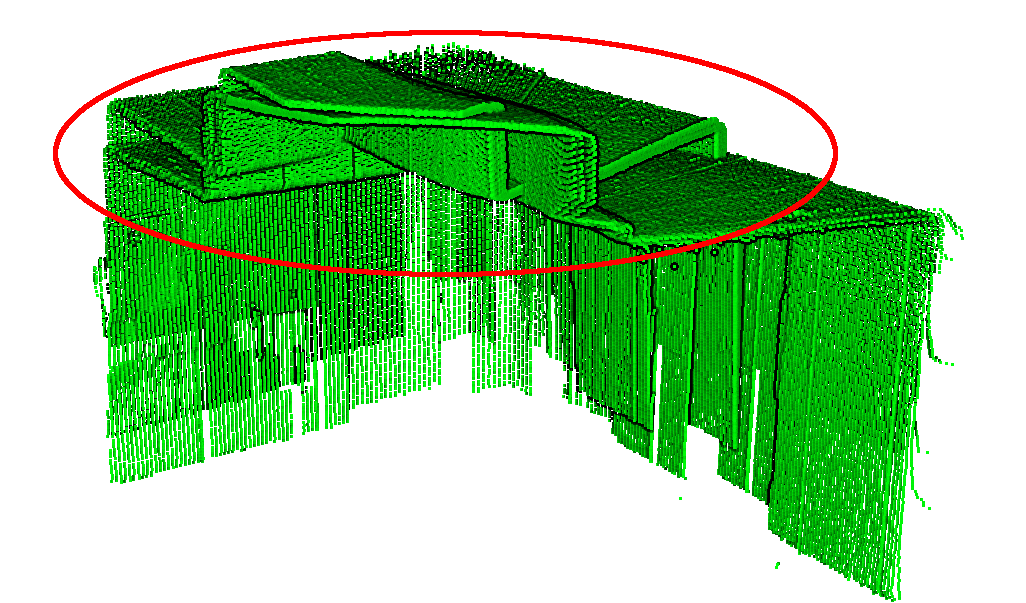
\includegraphics[width = 8cm]{images/example-pointcloud-2-bad}} \qquad
    \subfloat{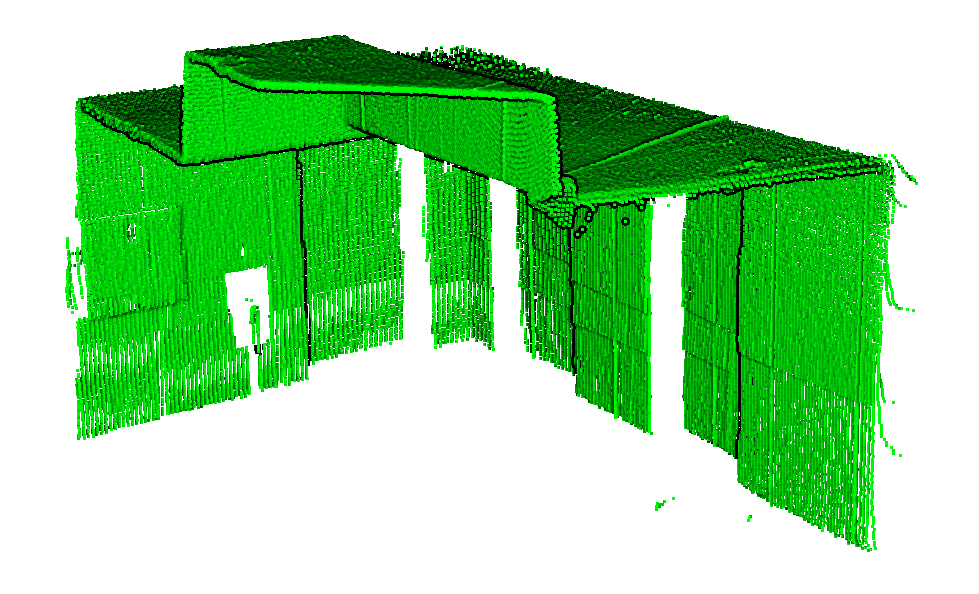
\includegraphics[width = 8cm]{images/example-pointcloud-2-good}}

    \centering
    \subfloat{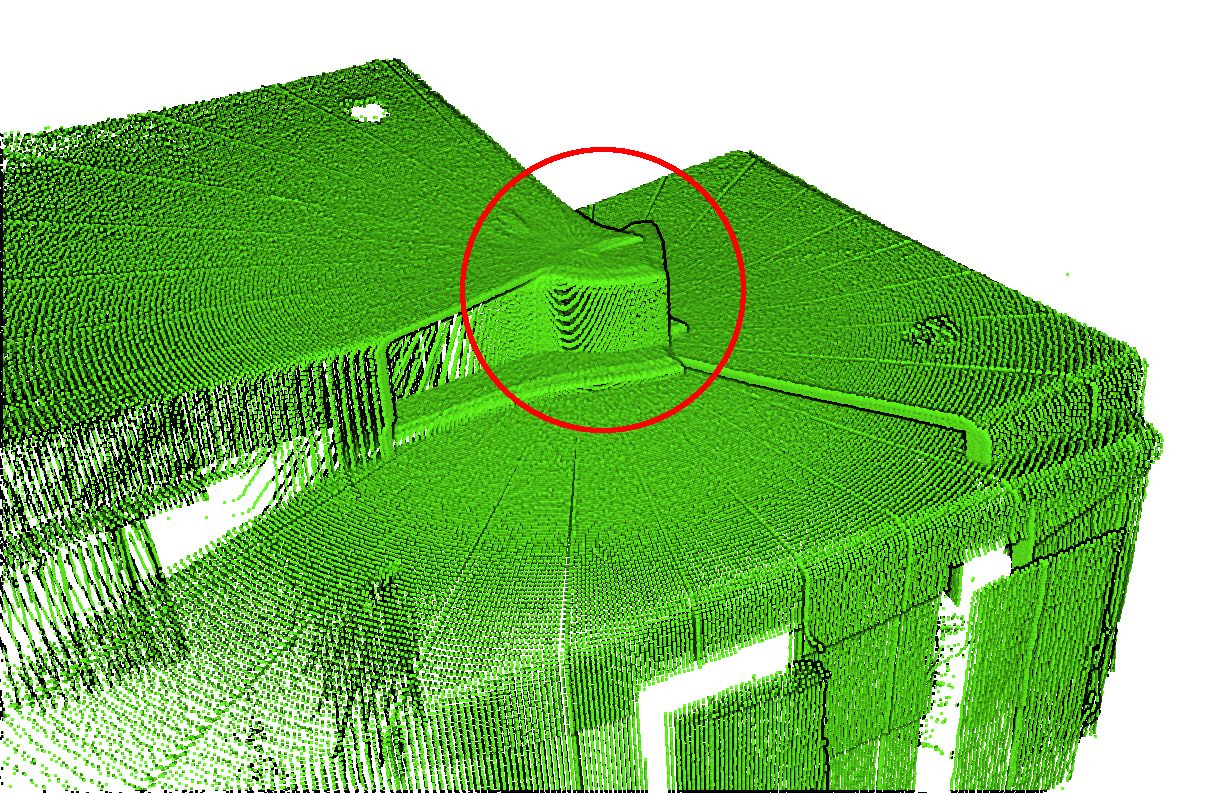
\includegraphics[width = 8cm]{images/example-pointcloud-3-bad}} \qquad
    \subfloat{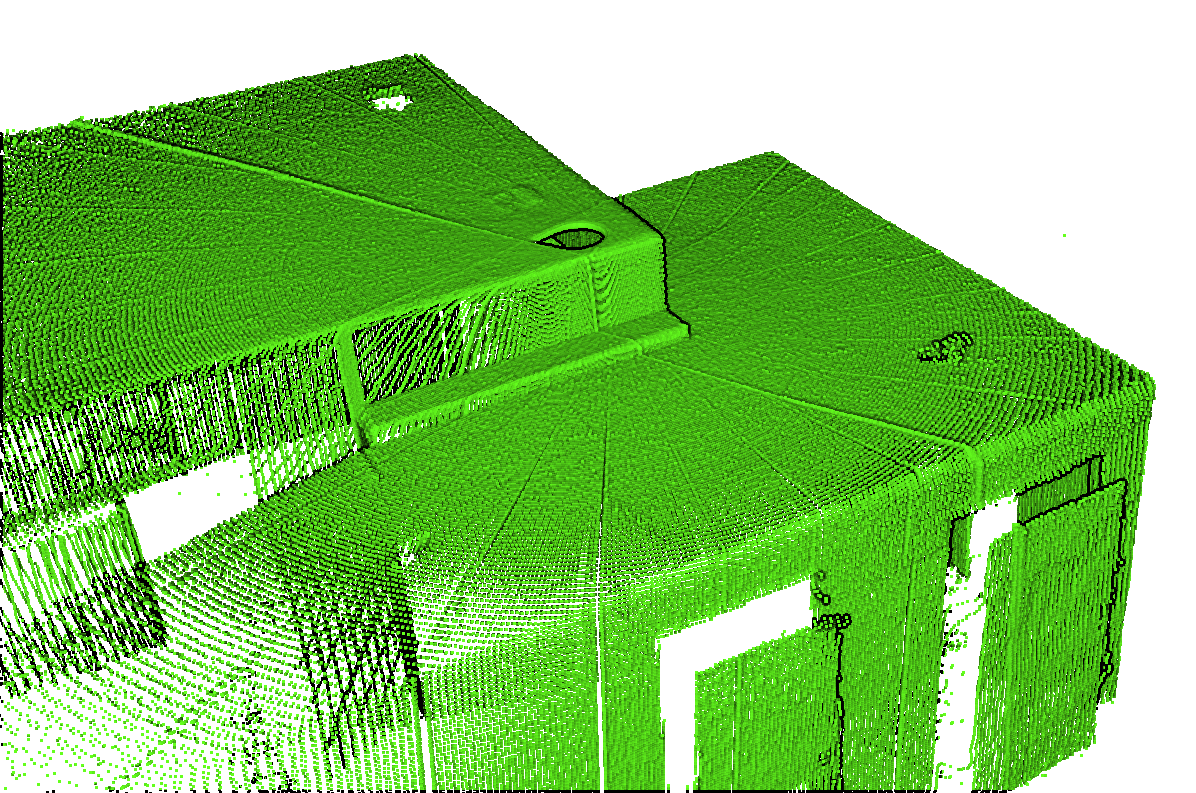
\includegraphics[width = 8cm]{images/example-pointcloud-3-good}}

    \centering
    \subfloat{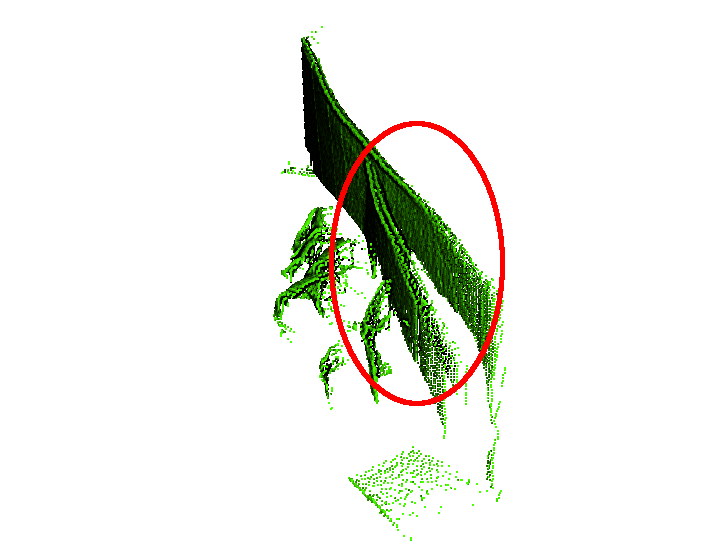
\includegraphics[height = 6cm]{images/example-pointcloud-1-bad}} \qquad
    \subfloat{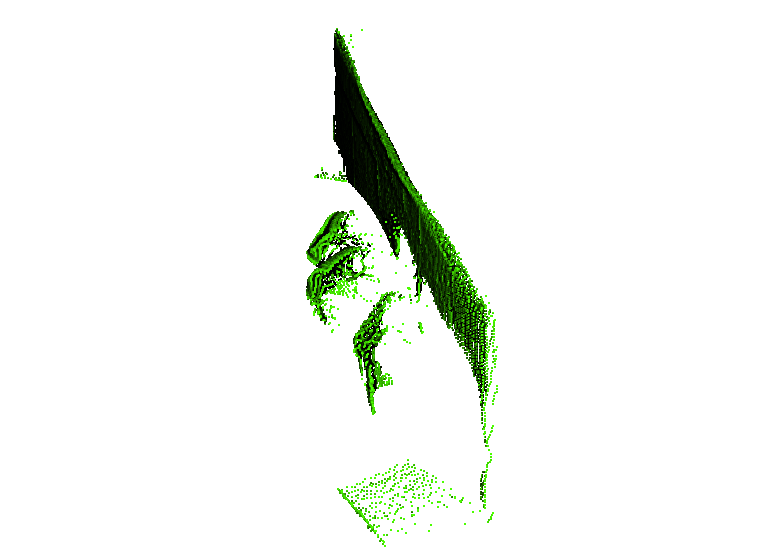
\includegraphics[height = 6cm]{images/example-pointcloud-1-good}}

    \caption{Side-by-side comparison of the uncalibrated (on the left) and calibrated (on the right) point clouds. The most noticeable distortions are marked in red, which did not appear in the calibrated point clouds. This indicated that the method successfully reduced the distortions in the point clouds.}
    \label{figure:visual-comparison}
\end{figure*}

Despite the good qualitative result shown prior, a further quantitative analysis was performed in order to evaluate the method. The results were prepared in the following steps:

\begin{itemize}
    \item A planar surface was extracted from both the calibrated and uncalibrated point cloud.
    \item The fitting plane was calculated for each surface, and the distance between the points to the surface was computed.
    \item The statistic deviation of the distances was calculated.
\end{itemize}

This method was performed for 3 planes, and the segments can be seen in \cref{table:quantitative-results}. As seen the statistical deviation is in fact smaller in the calibrated point cloud. As an alternative view, in \cref{figure:deviation-histogram}, the histogram and distribution of the signed deviation is shown for both the point clouds. As shown, the deviations of the calibrated point cloud are less scattered than the deviations of the uncalibrated point cloud. This results indicate that this calibration method in fact improves the results. 

\begin{table}
    \caption{Comparison between the standard deviation and mean of the distances of the points to the plane for both the calibrated and uncalibrated point clouds.}
    \begin{tabu}{X[l] X[c] X[c]}
        \toprule
        Point Cloud & $\mu$ (average) & $\sigma$ (std. dev.) \\
        \midrule
        Calibrated     & 0.0495 & 0.2589 \\
        Uncalibrated   & 0.0025 & 1.1211 \\
        \bottomrule
    \end{tabu}

    \label{table:quantitative-results}
\end{table}

\begin{figure}[h]
    \centering
    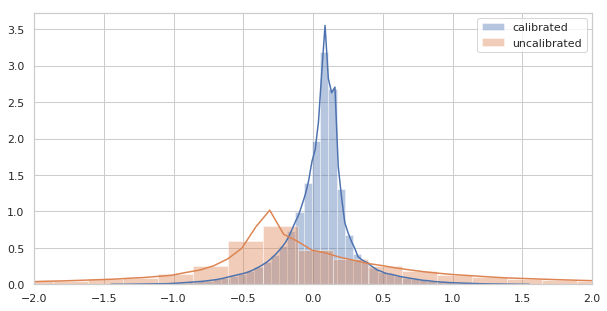
\includegraphics[width=8cm]{images/pointclouds-histogram.png}
    \caption{Distribution of the distances of the points to the plane. The uncalibrated points is a wider than the calibrated points, which indicates an improved calibration.}
    \label{figure:deviation-histogram}
\end{figure}


%%%%%%%%%%%%%%%%%%%%%%%%%%%%%%%%%%%%%%%%%%%%%%%%%%
\section{Conclusions and Future Work}\label{sec:conclusions}
%%%%%%%%%%%%%%%%%%%%%%%%%%%%%%%%%%%%%%%%%%%%%%%%%%

This paper presents a calibration procedure to determine the extrinsic transformation of LRF mounted on a robotic arm. This transformation is uttermost necessary for multiple applications, most noticeable, 3D reconstruction systems. The incorrect calibration of this systems results in artifacts and deformations on the final reconstructions, which invalidates any successive work in this point clouds. The proposed method is based on the measurement of the deformations of reconstructed planar surfaces, and through an optimization procedure, this deformations are minimized. The method was proved to be effective, through a visual inspection of the resulting point cloud and through a statistical evaluation of the reconstructed geometries.

\bibliographystyle{IEEEtran}
\bibliography{references/refs}


\end{document}
